
\section{Cross-point ReRAM Macro Design??}\label{sec:macro}
Since the array size of a cross-point ReRAM array is strictly limited by
reliability requirements, the design of a ReRAM macro is greatly different
from the traditional DRAM design. A cross-point ReRAM macro is implemented
by establishing a large amount of small cross-point arrays with
appropriate peripheral circuity and organizations. In this section, we
evaluate the area, energy consumption, and bandwidth of a 256 Mbits ReRAM
macro. We apply the similar memory organization as Kawahara's
work~\cite{crossbar_Panasonic}. The 256 Mbits ReRAM macro consists of
eight planes, each of which is 32 Mbits. Each plane has separate wordline
decoder, bitline selectors, sense amplifiers, and write circuity. Due to
limitations of space, we only present the results of ReRAM macro
implemented by four different typical cell parameters: ($Kr=20,
I_w=40uA$), ($Kr=20, I_w=200uA$), ($Kr=40, I_w=40uA$), and ($Kr=40,
I_w=200uA$). For each of them, we vary the number of bit per write to
investigate the relation among the area, energy consumption, and bandwidth
of the ReRAM macro.


%Figure~\ref{fig:aaable}
Figure~14 shows the total area, energy consumption, and bandwidth of the
256 Mbits ReRAM macro. Clearly, consistent to our previous discussion, the
total area and energy consumption of the ReRAM macro increase with the
increase of nonlinearity, the scaling of write current, as well as the
increase of the number of array-level bits per write. Besides, the
bandwidth also has the similar trend as area and energy consumption. This
observation implies that we have to either sacrifice the area efficiency
or increase the energy budget to improve the bandwidth of the ReRAM macro.

The bandwidth-per-Joule is another important measurement of the energy
efficiency of the memory macro. Figure~\ref{fig:EpJ} shows the
bandwidth-per-Joule of the ReRAM macro. For a certain ReRAM cell, the
single-bit write operation always has the best bandwidth-per-Joule value.
It is because the multi-bit write operation requires a two-step write
method, which almost doubles the latency of write operation and therefore
impact the bandwidth-per-Joule value. Besides, for the multi-bit write
operation, the bandwidth-per-Joule do not increase monotonically with the
increase of the number of bit per write. According to
Figure~\ref{fig:EpJ}, an optimal write scheme exists for each of the
different cell parameters. For example, for our baseline design with
$Kr=20$ and $I_w=40uA$, write 32 bits per access will result in the best
bandwidth-per-Joule value. Therefore, to design a bandwidth-per-Joule
efficient ReRAM macro, the optimal scheme should be carefully decided.


\begin{figure}[!t]
\centering\label{fig:aaable}
  % Requires \usepackage{graphicx}
  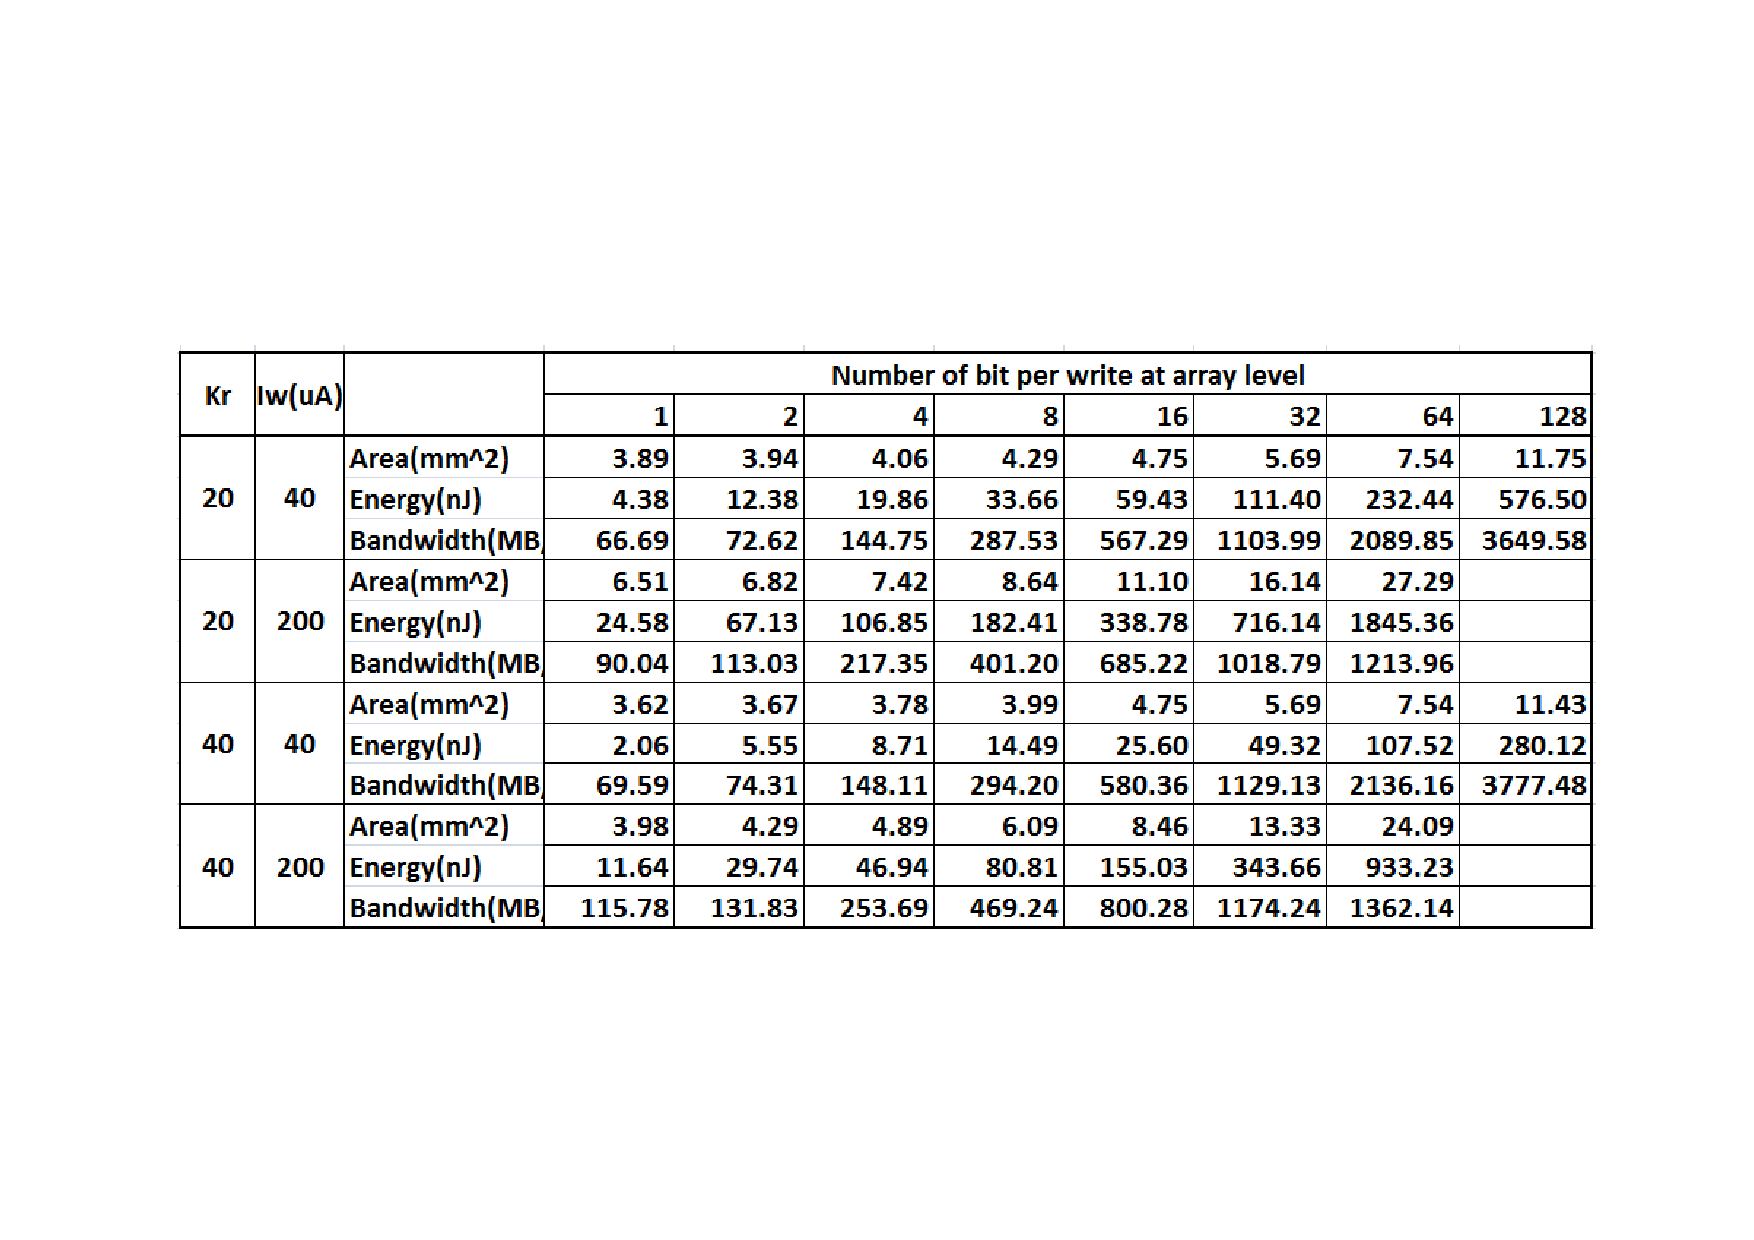
\includegraphics[width=0.5\textwidth]{./figures/Table}\\
  \caption{Area, energy, and bandwidth results of 256 Mbits ReRAM macro.}
  \vspace{-5pt}
\end{figure}


\begin{figure}[!t]
\centering\label{fig:EpJ}
  % Requires \usepackage{graphicx}
  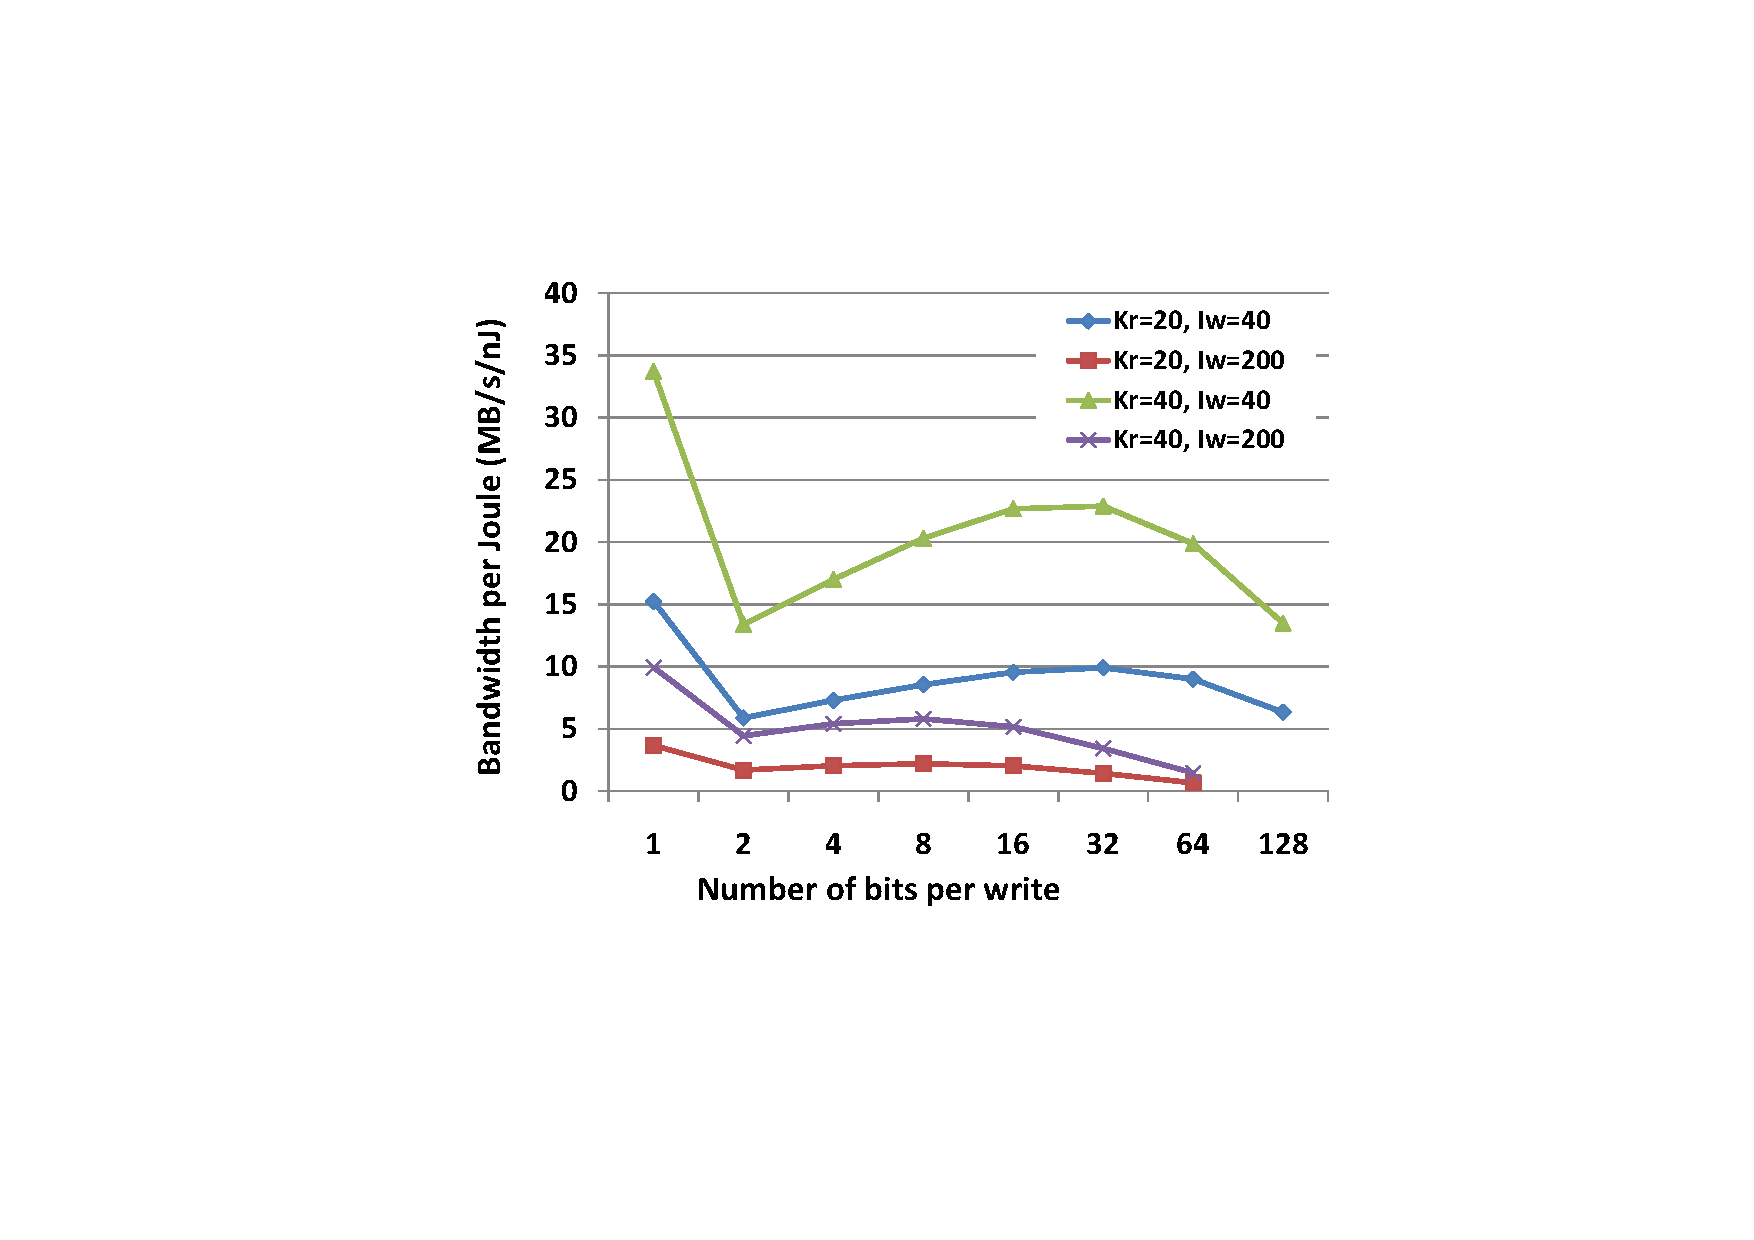
\includegraphics[width=0.4\textwidth]{./figures/EpJ}\\
  \caption{Bandwidth-per-Joule of 256 Mbits ReRAM macro.}
  \vspace{-5pt}
\end{figure}

%\begin{table}
%\begin{tabular}{|l|l||l|l|l|l|l|l|l|l|}
%\hline
%\multicolumn{8}{|c|}{Num of bit per write}\\
%$Kr$ & $I_w$ & 1 & 2 & 4 & 8 & 16 & 32 & 64 & 128 \\\hline
%\multirow{3}{*}{20} & \multirow{3}{*}{20} & & ~ & ~ & ~ & ~ & ~ & ~ & ~ & ~ \\
%& ~ & ~ & ~ & ~ & ~ & ~ & ~ & ~
%& ~ & ~ & ~ & ~ & ~ & ~ & ~ & ~\\\hline
%20 & ~ & ~ & ~ & ~ & ~ & ~ & ~ & ~ & ~ \\\hline
%20 & ~ & ~ & ~ & ~ & ~ & ~ & ~ & ~ & ~ \\\hline
%20 & ~ & ~ & ~ & ~ & ~ & ~ & ~ & ~ & ~ \\\hline
%40 & ~ & ~ & ~ & ~ & ~ & ~ & ~ & ~ & ~ \\\hline
%40 & ~ & ~ & ~ & ~ & ~ & ~ & ~ & ~ & ~ \\\hline
%40 & ~ & ~ & ~ & ~ & ~ & ~ & ~ & ~ & ~ \\\hline
%40 & ~ & ~ & ~ & ~ & ~ & ~ & ~ & ~ & ~ \\\hline
%40 & ~ & ~ & ~ & ~ & ~ & ~ & ~ & ~ & ~ \\\hline
%40 & ~ & ~ & ~ & ~ & ~ & ~ & ~ & ~ & ~ \\\hline
%40 & 200 & ~ & ~ & ~ & ~ & ~ & ~ & ~ & ~ \\
%\end{tabular}
%\end{table}
